\documentclass[12pt, a4]{report}
    \usepackage[utf8]{inputenc}
    \usepackage[croatian]{babel}
    \usepackage{graphicx}
    \usepackage[a4paper, total={6in, 10in}]{geometry}
    \usepackage{caption}
    \usepackage{amsmath}
    \usepackage{subfig}
    \usepackage{siunitx}

    \graphicspath{ {res/} }

    \title{Laboratorijska vježba 4}
    \author{Matija Marić, 0036479678}
    \date{\today}

\begin{document}
\begin{titlepage}
	\maketitle
\end{titlepage}

\tableofcontents{}

\chapter{Segmentacija slike}
\section{Amplitudna segmentacija}
\subsection{Ručno odabiranje praga}

\begin{enumerate}
	\item 
		\begin{minipage}{\linewidth}
			\centering
			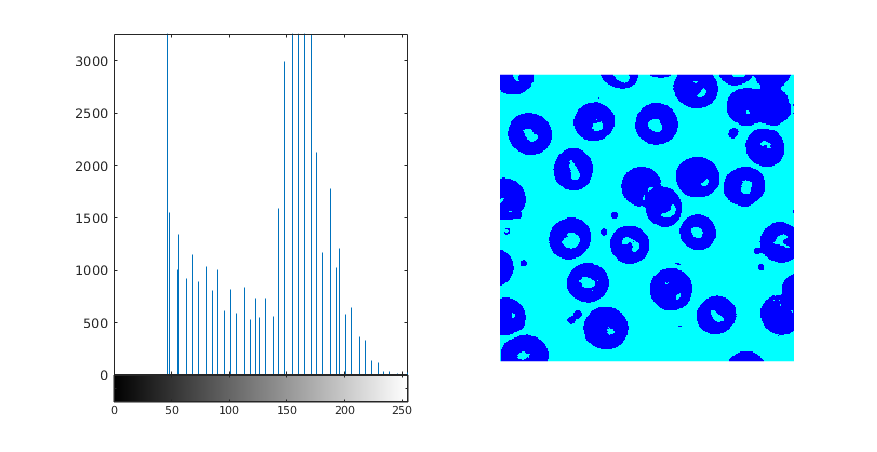
\includegraphics[width=0.75\textwidth]{histslice}
			\captionof{figure}{Slika {\it blood1.tif} segmentirana prema pragu histograma na razini 130.}
		\end{minipage}
	\item 
		\begin{minipage}{\linewidth}
			\centering
			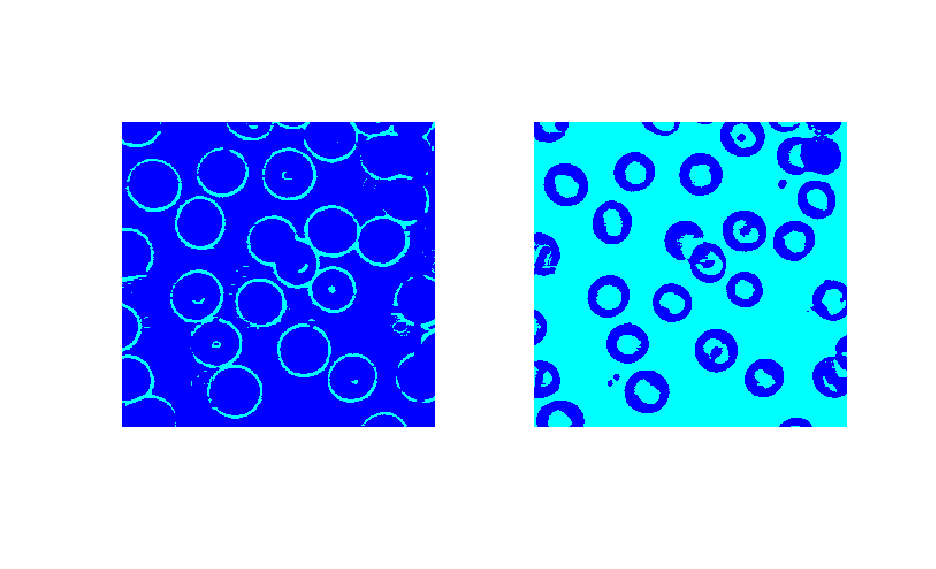
\includegraphics[width=0.75\textwidth]{histplusmin}
			\captionof{figure}{Slika {\it blood1.tif} segmentirana sa pragom +0.2 i -0.2 od optimalne razine praga. Povećanjem praga ostaju samo vanjski rubovi, a smanjenjem se gube dijelovi unutrašnjosti.}
		\end{minipage}
	\item 
		\begin{minipage}{\linewidth}
			\centering
			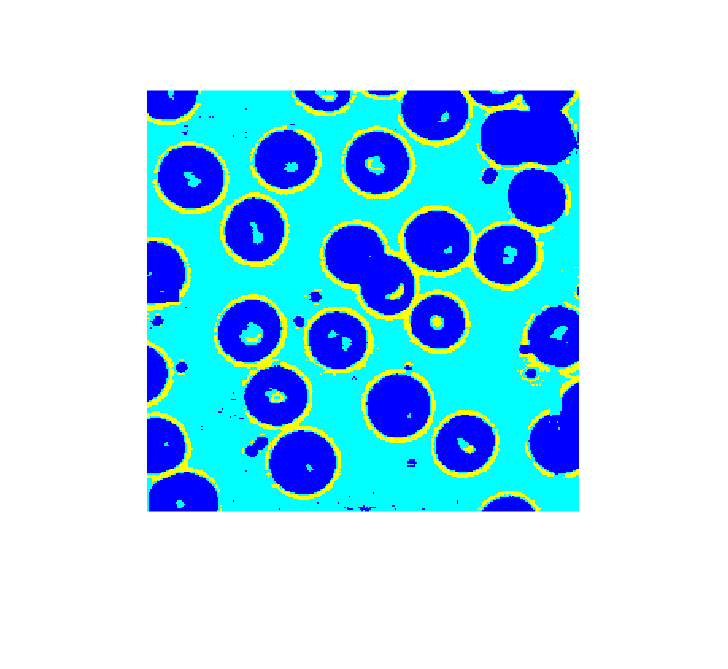
\includegraphics[width=0.75\textwidth]{histtrimodal}
			\captionof{figure}{Slika {\it blood1.tif} segmentirana na pragovima histograma 140 i 180. Dobiveni su zasebno segmentirani rubovi i unutrašnjost stanica.}
		\end{minipage}
\end{enumerate}

\subsection{Automatsko odabiranje praga}

\begin{enumerate}
	\item 
		\begin{minipage}{\linewidth}
			\centering
			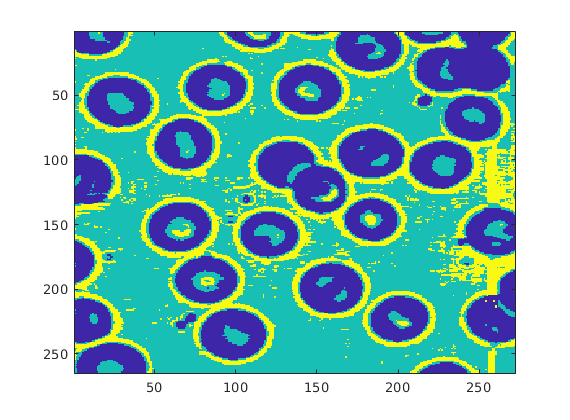
\includegraphics[width=0.75\textwidth]{kmeans}
			\captionof{figure}{Slika {\it blood1.tif} segmentirana automatski određenim pragovima algoritmom K-sredina. Dobiveni pragovi su [0.2291, 0.6012, 0.7305]. K-means određuje najzastupljenije grupe i zato ostaje dosta šuma, ako ručno zadamo pragove možemo smanjiti količinu šuma.}
		\end{minipage}
\end{enumerate}

\section{Određivanje rubova}

\begin{enumerate}
	\item 
		\begin{minipage}{\linewidth}
			\centering
			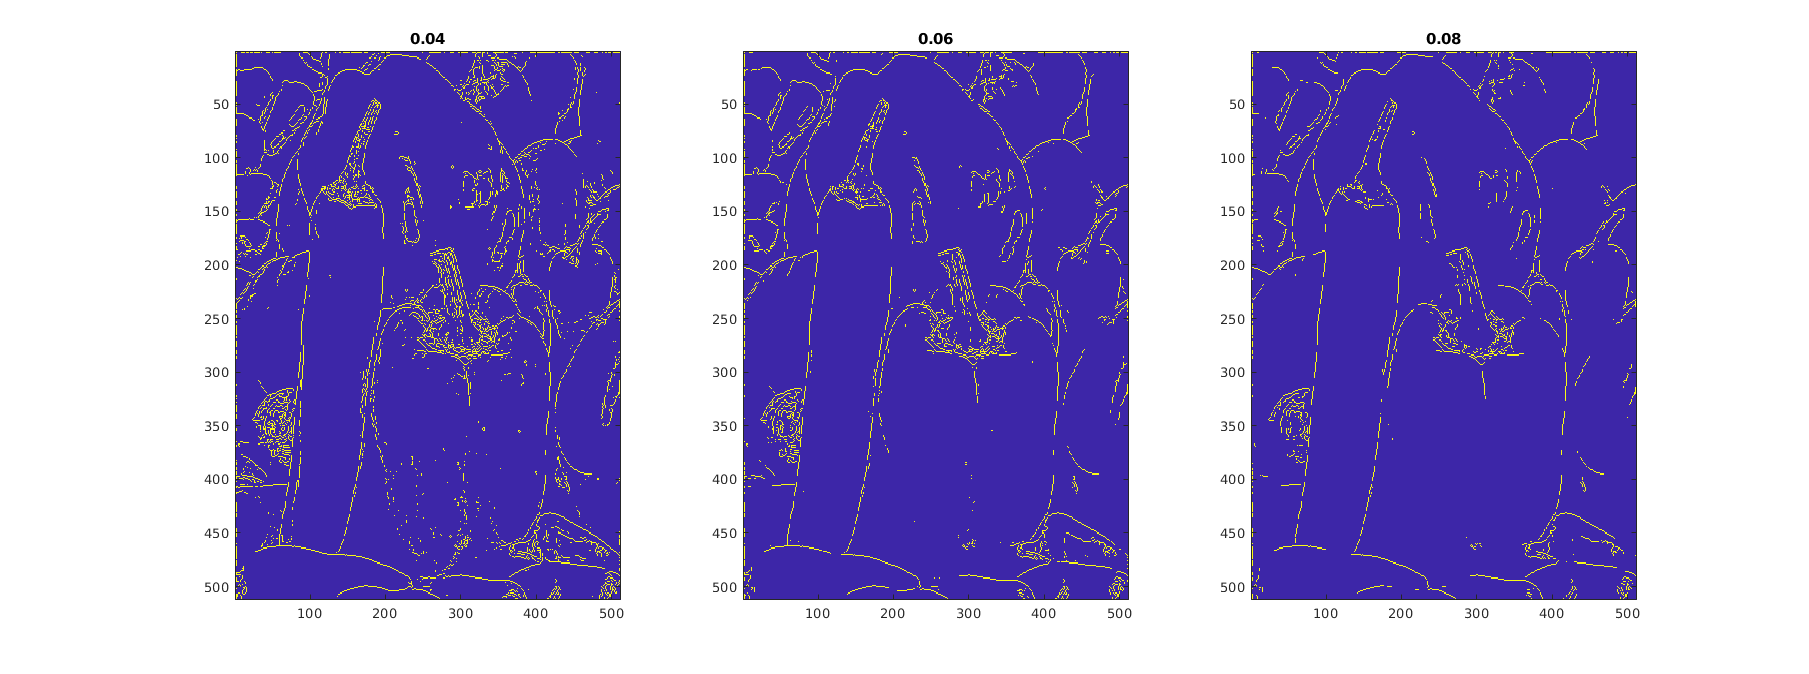
\includegraphics[width=0.75\textwidth]{sobelparam}
			\captionof{figure}{Rubovi slike {\it 4.2.07.tiff} određeni Sobelovim operatorom sa različitim vrijednostima praga. Najbolji je slučaj sa pragom 0.08, jer je najmanja količina šuma.}
		\end{minipage}
	\item 
		\begin{minipage}{\linewidth}
			\centering
			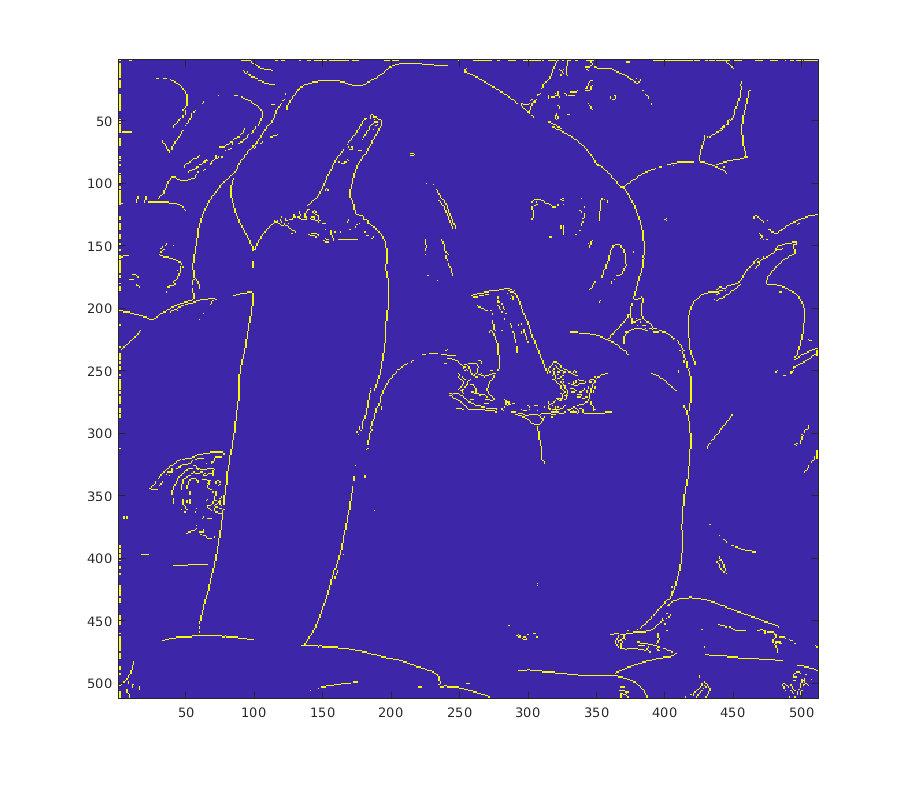
\includegraphics[width=0.75\textwidth]{sobelauto}
			\captionof{figure}{Rubovi slike {\it 4.2.07.tiff} određeni Sobelovim operatorom sa automatski određenim pragom. Dobiveni rezultat je blizu onoga sa ručno određenim pragom 0.08, ali su rubovi manje isprekidani.}
		\end{minipage}
	\item 
		\begin{minipage}{\linewidth}
			\centering
			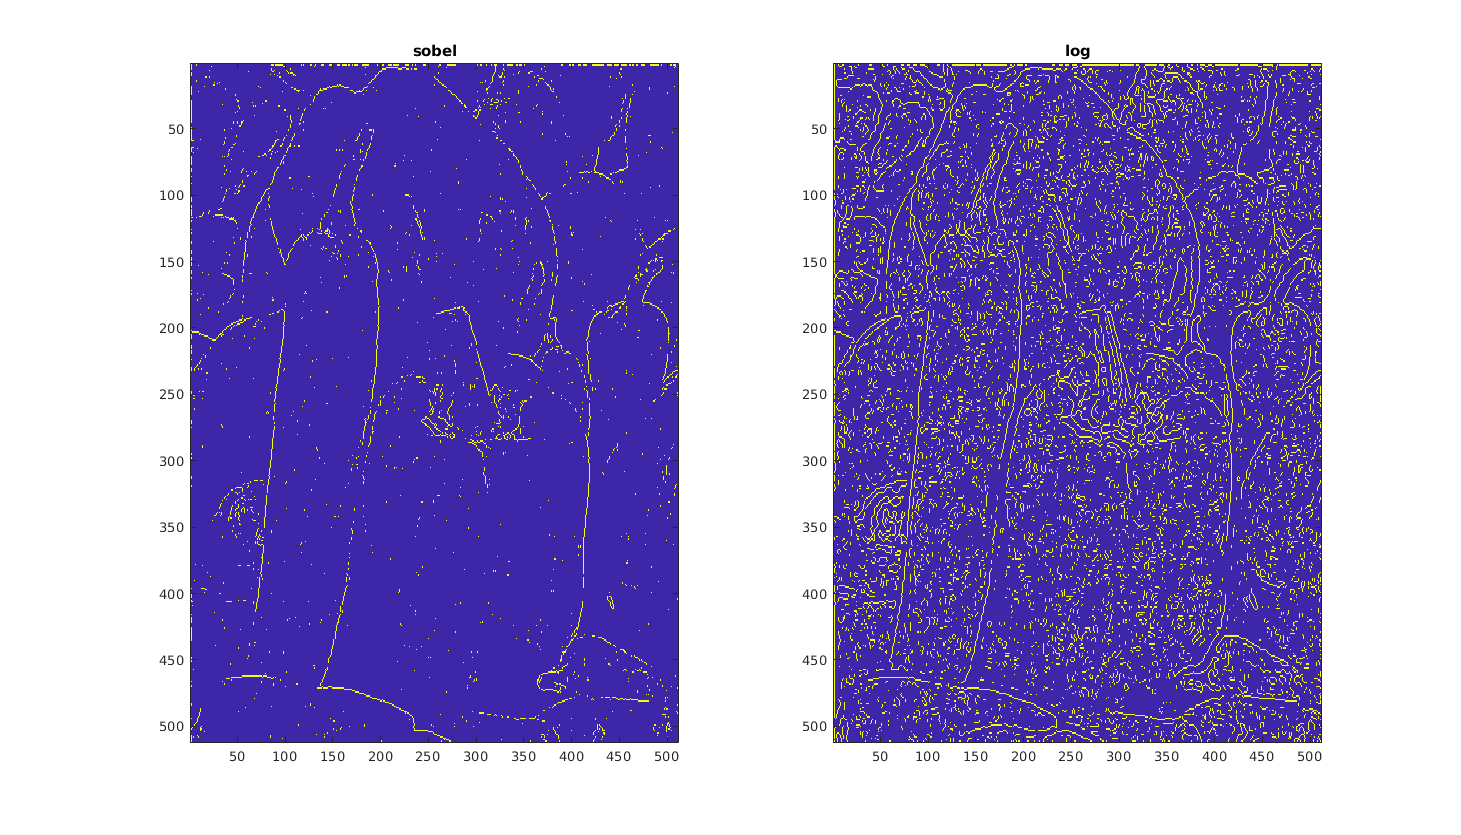
\includegraphics[width=0.75\textwidth]{edgenoise}
			\captionof{figure}{Usporedba detekcije rubova na slici {\it 4.2.07.tiff} sa dodanim Gaussovim šumom, sa Sobelovim operatorom i log metodom. Sobel puno bolje podnosi šum na slici.}
		\end{minipage}
	\item 
		\begin{minipage}{\linewidth}
			\centering
			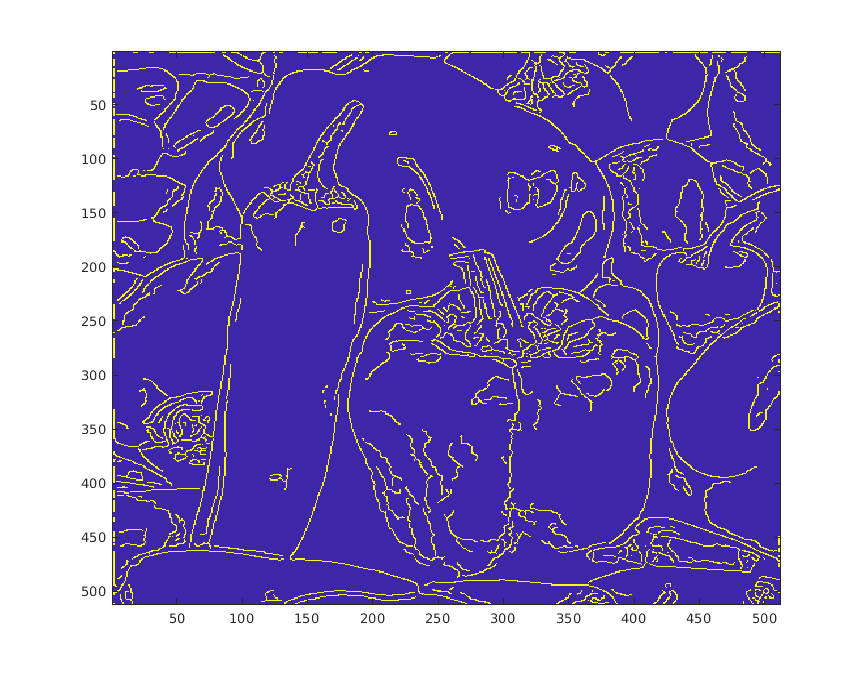
\includegraphics[width=0.75\textwidth]{canny}
			\captionof{figure}{Detekcija rubova Cannyevom metodom na slici {\it 4.2.07.tiff}. Rubovi su bolje detektirani od ostalih metoda, kontinuirani su i mala je količina šuma.}
		\end{minipage}
\end{enumerate}

\section{Segmentacija tekstura}

\begin{enumerate}
	\item 
		\begin{minipage}{\linewidth}
			\centering
			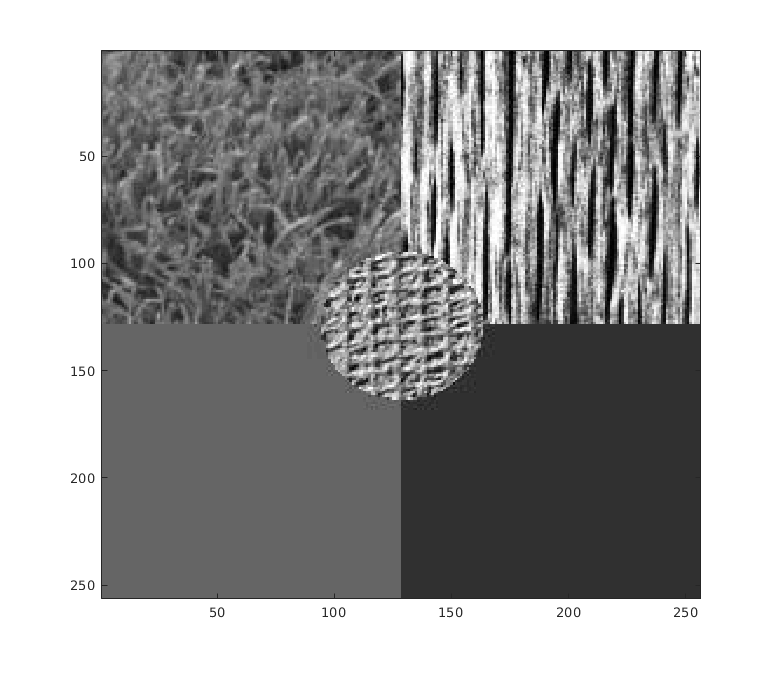
\includegraphics[width=0.75\textwidth]{texture}
			\captionof{figure}{Slika {\it texture.tif}, ima 5 različitih tekstura. Prva tekstura nema nekog jasnog uzorka, druga tekstura i ona u centru imaju uzorak, a druge dvije su uniformne.}
		\end{minipage}
	\item 
		\begin{minipage}{\linewidth}
			\centering
			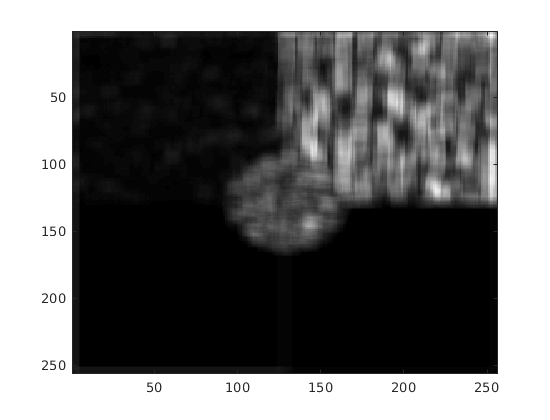
\includegraphics[width=0.75\textwidth]{texturefeats}
			\captionof{figure}{Značajke na {\it texture.tif} određene funkcijom \texttt{inertia}.}
		\end{minipage}
		\begin{minipage}{\linewidth}
			\centering
			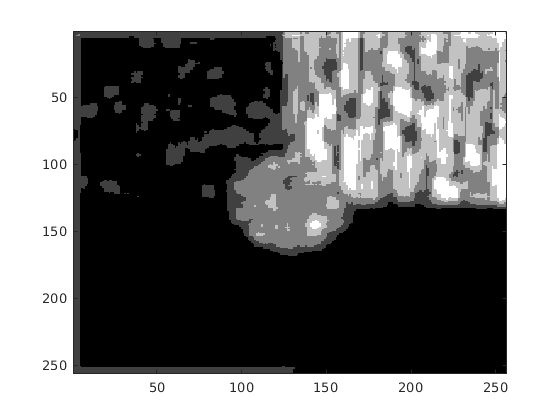
\includegraphics[width=0.75\textwidth]{texturekmeans}
			\captionof{figure}{Značajke na {\it texture.tif} određene funkcijom \texttt{inertia} segmentirane metodom K-sredina. }
		\end{minipage}
	\item 
		\begin{minipage}{\linewidth}
			\centering
			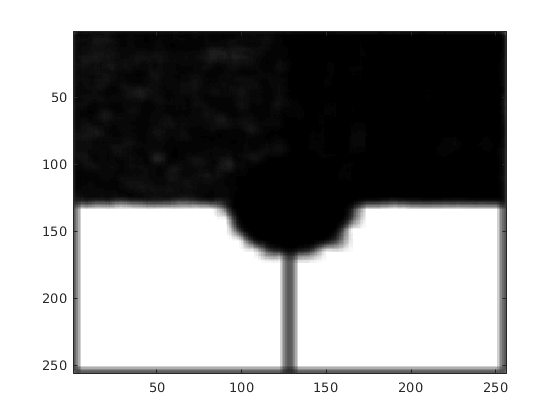
\includegraphics[width=0.75\textwidth]{textureenergy}
			\captionof{figure}{Energija spektra na slici {\it texture.tif}}
		\end{minipage}
		\begin{minipage}{\linewidth}
			\centering
			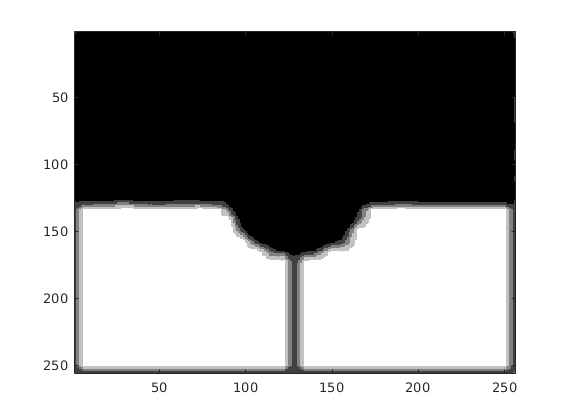
\includegraphics[width=0.75\textwidth]{energykmeans}
			\captionof{figure}{Slika {\it texture.tif} segmentirana prema energiji spektra. Ova metoda je dobra kod određivanja uniforminih tekstura.}
		\end{minipage}
\end{enumerate}

\chapter{Registracija slike}
\section{Registracija slike}

\begin{enumerate}
	\item 
		\begin{minipage}{\linewidth}
			\centering
			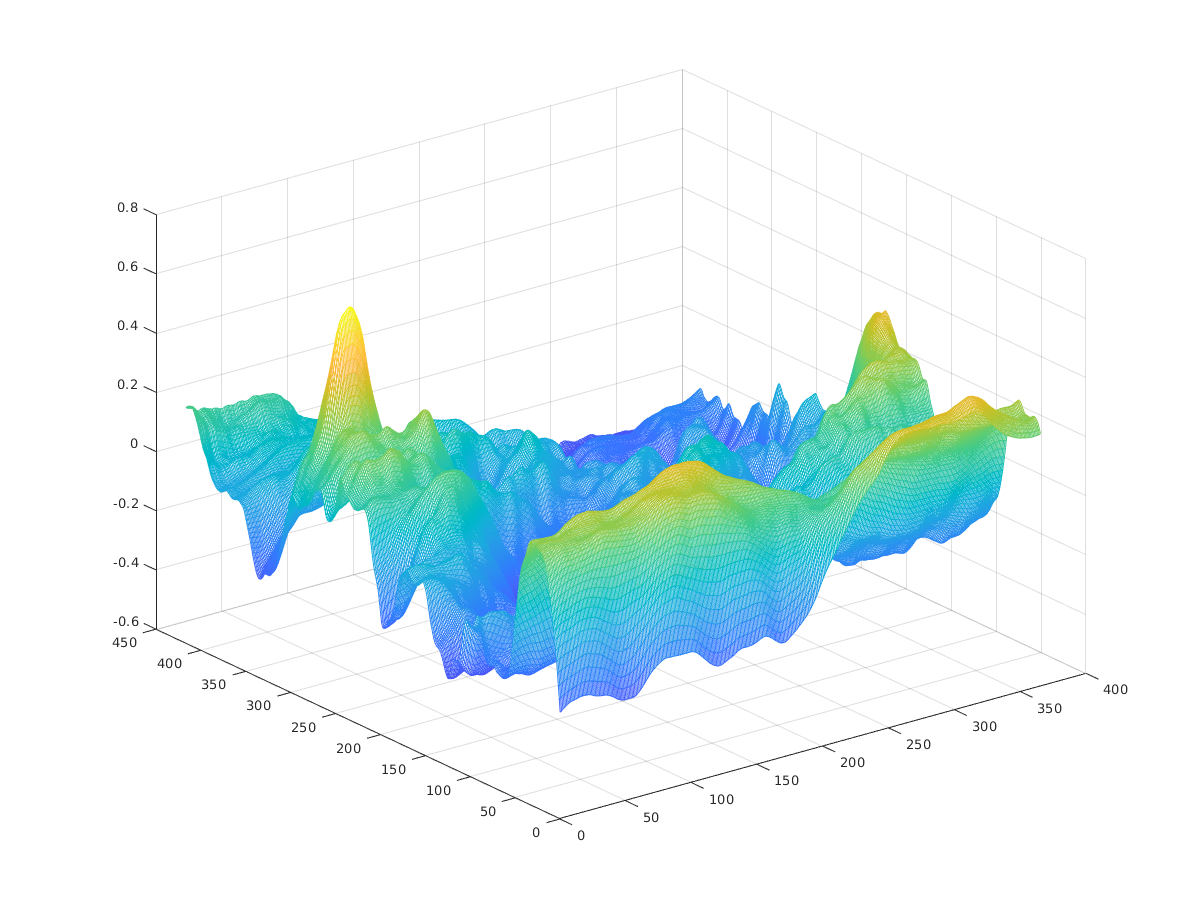
\includegraphics[width=0.75\textwidth]{correlation}
			\captionof{figure}{Korelacijska matrica za slike {\it auto1.tiff} i {\it slika1.tiff}.}
		\end{minipage}
	\item
		Maksimum matrice je u (294, 41).
	\item 
		\begin{minipage}{\linewidth}
			\centering
			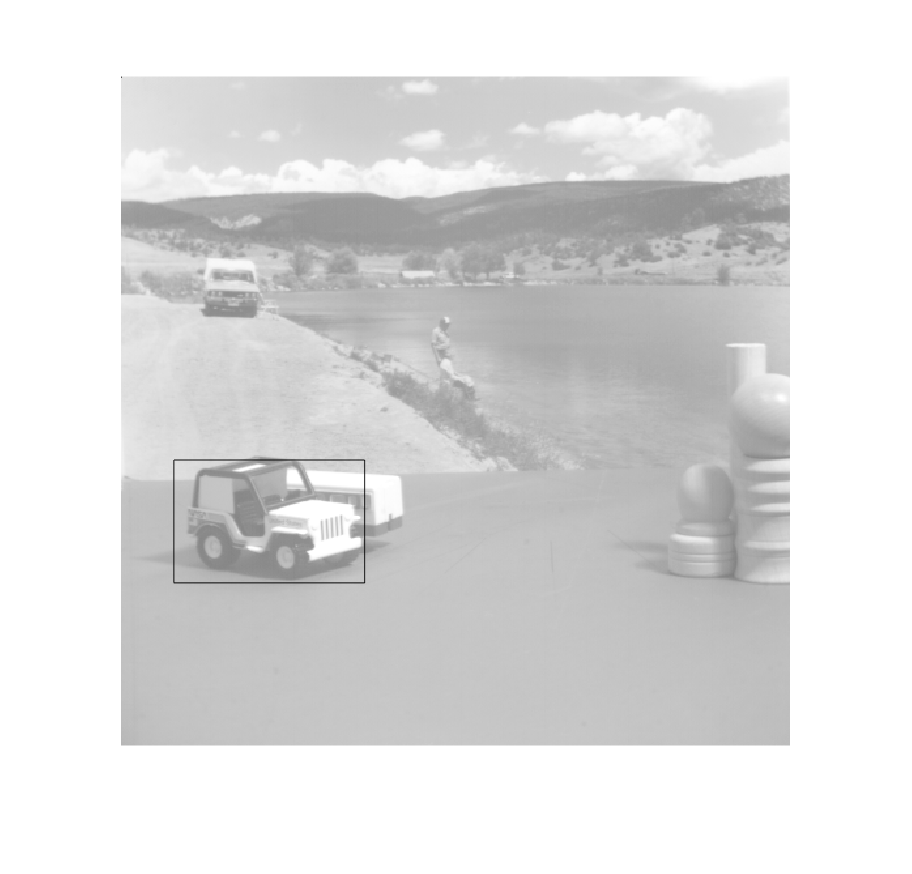
\includegraphics[width=0.75\textwidth]{corrreg}
			\captionof{figure}{Označen pravokutnik na položaju maksimalne korelacije na slici {\it slika1.tiff}}
		\end{minipage}
	\item 
		\begin{minipage}{\linewidth}
			\centering
			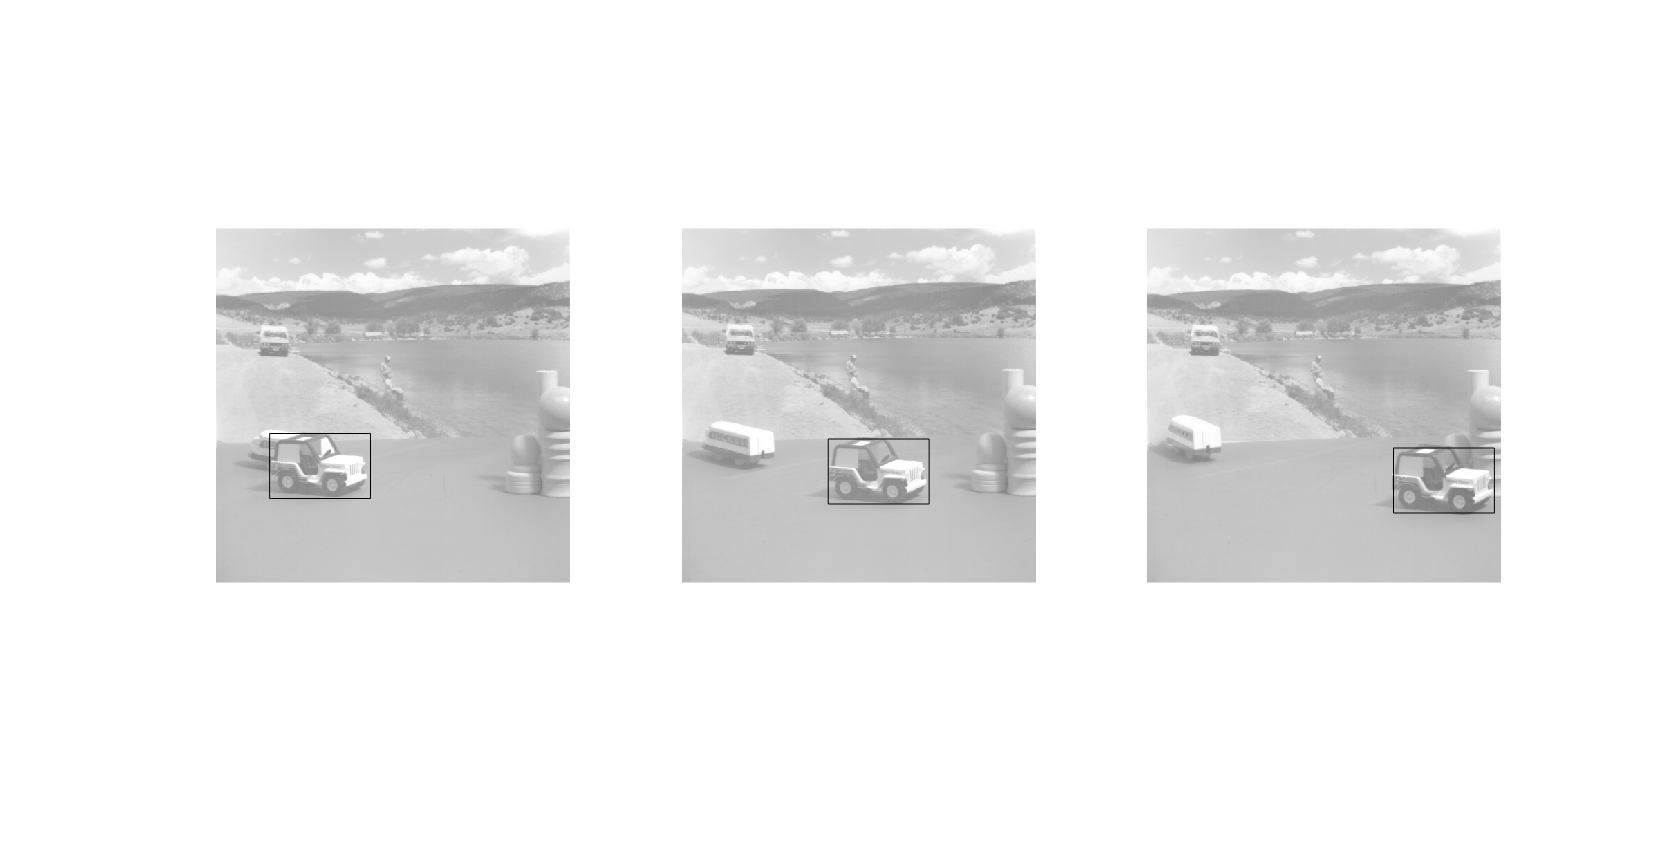
\includegraphics[width=0.75\textwidth]{objectdetect}
			\captionof{figure}{Detekcija objekta na slikama {\it slika1.tiff}, {\it slika2.tiff}, {\it slika3.tiff}}
		\end{minipage}
	\item 
		\begin{minipage}{\linewidth}
			\centering
			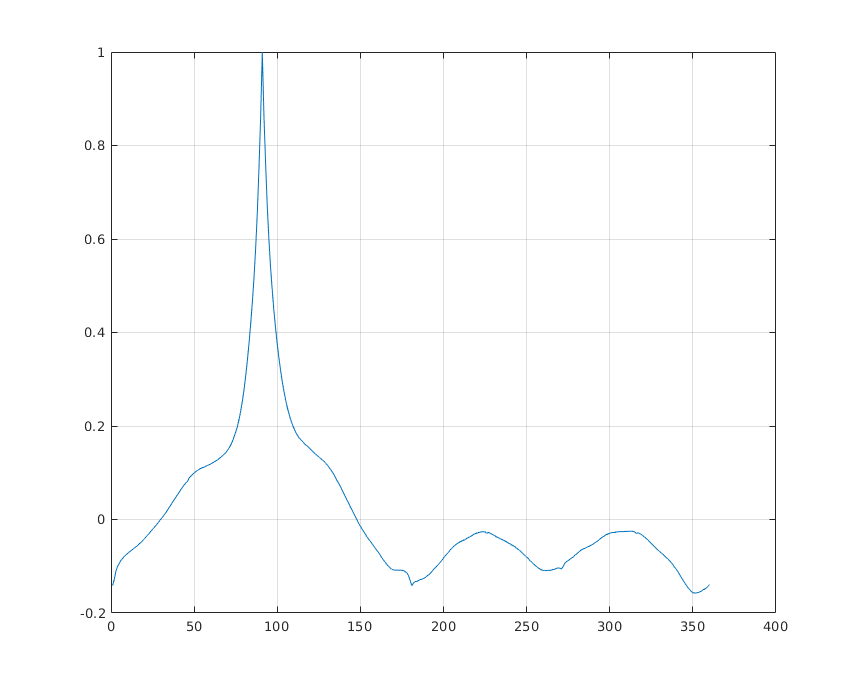
\includegraphics[width=0.75\textwidth]{rotationcor}
			\captionof{figure}{Korelacija slika {\it auto1.tiff} i {\it auto2.tiff} s obzirom na rotaciju jedne od slika. Najveća je korelacija za kut \ang{90}. }
		\end{minipage}
	
\end{enumerate}

\end{document}